% make sure to download following files before compiling-
% tikzlibrarynode-families.code.tex
% tikzlibrarypositioning-plus.code.tex
% please keep the above files in the same directory
\documentclass[11pt]{beamer}

\usepackage[whole]{bxcjkjatype} % For Japanese language

\usefonttheme{serif}
\usepackage{graphicx}
\usepackage{tikz}
\usetikzlibrary{shapes.geometric,backgrounds,positioning-plus,node-families,calc}
\tikzset{
  basic box/.style = {
    shape = rectangle,
    align = center,
    draw  = #1,
    fill  = #1!25,
    font  = \Large,
    rounded corners},
  header node/.style = {
    %Minimum Width = header nodes,
    font          = \huge\bf,
    text depth    = +0pt,
    fill          = white,
    draw},
  header/.style = {%
    inner xsep = +1.2em,
    inner ysep = +1.5em,
    append after command = {
      \pgfextra{\let\TikZlastnode\tikzlastnode}
      node [header node] (header-\TikZlastnode) at (\TikZlastnode.north) {#1}
      node [span = (\TikZlastnode)(header-\TikZlastnode)]
        at (fit bounding box) (h-\TikZlastnode) {}
    }
  },
  hv/.style = {to path = {-|(\tikztotarget)\tikztonodes}},
  vh/.style = {to path = {|-(\tikztotarget)\tikztonodes}},
  fat blue line/.style = {ultra thick, blue}
}
\setbeamertemplate{navigation symbols}{}
\setbeamersize{text margin left=0.2em,text margin right=0.2em}

\begin{document}
\begin{frame}
%\hskip -2em
\begin{tikzpicture}[scale=0.48, every node/.style={transform shape}, thick, >=latex]
	\node[basic box=blue, header=Teaching Phase] (teaching) {
		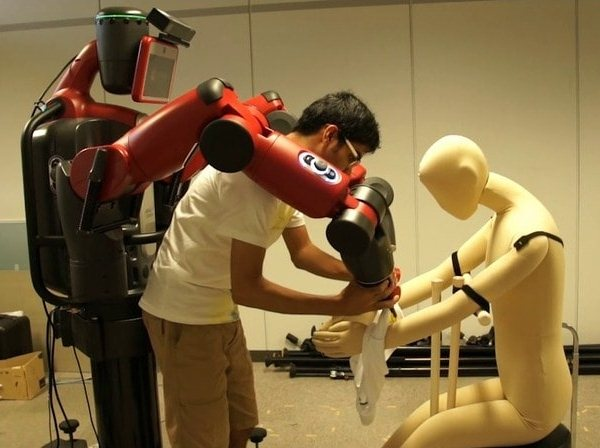
\includegraphics[width=8cm]{teaching_new}\\
		%A demonstration is performed by moving the \\
		%Baxter arms in the appropriate trajectory
		デモンストレーションはBaxter の両腕を\\
		適切な軌道にそって動かすことで行われる.
	};
	
	\node[north right=of teaching, basic box=orange, header=Learn Trajectory, shift=(right:1.2*x_node_dist)] (dmp) {
		Baxter Left Arm Trajectory\\
		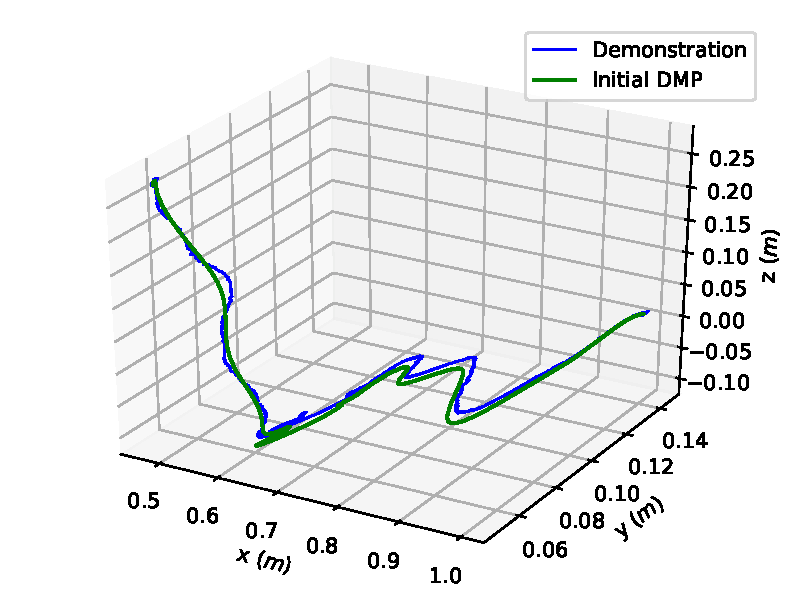
\includegraphics[height=6cm]{dmp_init}\\
		%Recorded trajectory is parameterized by DMP
		DMPによってパラメータ化された軌道を保存する
	};
		
	\node[east below=of teaching, basic box=red, header=DMP Generalization, shift=(right:1.2*x_node_dist)] (generalization){
		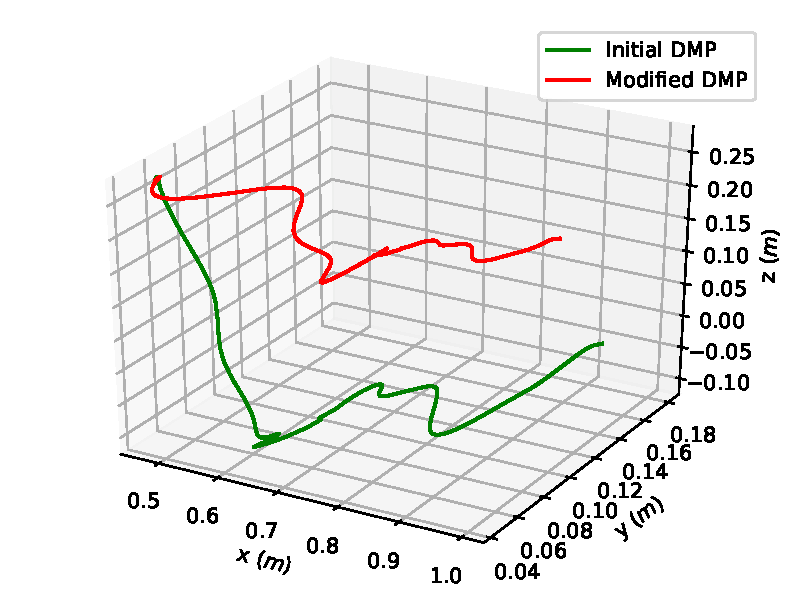
\includegraphics[height=6cm]{dmp_mod}\\
		%Arms posture of the mannequin is changed.\\
		%Accordingly goal parameter of DMP is modified
		マネキンの腕の姿勢が変更する. \\
		これに応じてDMPのゴールパラメータは修正される
	};

	\node[north right=of generalization, basic box=green, header=Testing Phase] (testing) {
		Modified Posture\\
		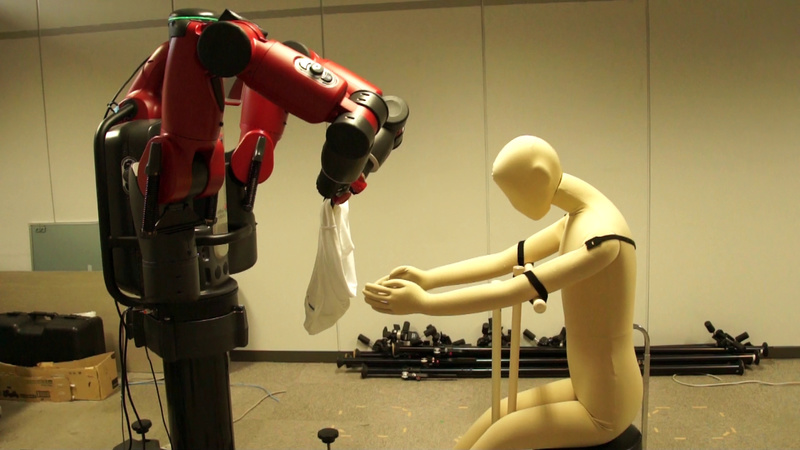
\includegraphics[width=10cm]{testing}\\
		%DMP can accomodate any posture by \\
		%changing goal parameter
		DMPはゴールパラメータを修正することで\\
		任意の姿勢に適応可能である
	};
	
	
    \path[ultra thick, blue, ->](teaching) edge[->] (dmp);
	\path[ultra thick, orange, ->](dmp) edge[->] (generalization);
	\path[ultra thick, green, ->](generalization) edge[->] (testing);
\end{tikzpicture}
\end{frame}
\end{document}
